
%% Beginning of file 'sample63.tex'
%%
%% Modified 2019 June
%%
%% This is a sample manuscript marked up using the
%% AASTeX v6.3 LaTeX 2e macros.
%%
%% AASTeX is now based on Alexey Vikhlinin's emulateapj.cls 
%% (Copyright 2000-2015).  See the classfile for details.

%% AASTeX requires revtex4-1.cls (http://publish.aps.org/revtex4/) and
%% other external packages (latexsym, graphicx, amssymb, longtable, and epsf).
%% All of these external packages should already be present in the modern TeX 
%% distributions.  If not they can also be obtained at www.ctan.org.

%% The first piece of markup in an AASTeX v6.x document is the \documentclass
%% command. LaTeX will ignore any data that comes before this command. The 
%% documentclass can take an optional argument to modify the output style.
%% The command below calls the preprint style which will produce a tightly 
%% typeset, one-column, single-spaced document.  It is the default and thus
%% does not need to be explicitly stated.
%%
%%
%% using aastex version 6.3
\documentclass[twocolumn]{aastex63}

\usepackage{amsmath}
\usepackage{empheq}
\usepackage{mathrsfs}
\usepackage{textcomp}
\usepackage{enumitem}   
\usepackage{gensymb}
\usepackage{hyperref}
\usepackage{graphicx}
\usepackage[caption=false]{subfig}
\usepackage{multirow}
\usepackage{longtable}
\hypersetup{colorlinks, linkcolor={blue}, citecolor={blue}, urlcolor={blue}} 
%% The default is a single spaced, 10 point font, single spaced article.
%% There are 5 other style options available via an optional argument. They
%% can be invoked like this:
%%
%% \documentclass[arguments]{aastex63}
%% 
%% where the layout options are:
%%
%%  twocolumn   : two text columns, 10 point font, single spaced article.
%%                This is the most compact and represent the final published
%%                derived PDF copy of the accepted manuscript from the publisher
%%  manuscript  : one text column, 12 point font, double spaced article.
%%  preprint    : one text column, 12 point font, single spaced article.  
%%  preprint2   : two text columns, 12 point font, single spaced article.
%%  modern      : a stylish, single text column, 12 point font, article with
%% 		  wider left and right margins. This uses the Daniel
%% 		  Foreman-Mackey and David Hogg design.
%%  RNAAS       : Preferred style for Research Notes which are by design 
%%                lacking an abstract and brief. DO NOT use \begin{abstract}
%%                and \end{abstract} with this style.
%%
%% Note that you can submit to the AAS Journals in any of these 6 styles.
%%
%% There are other optional arguments one can invoke to allow other stylistic
%% actions. The available options are:
%%
%%   astrosymb    : Loads Astrosymb font and define \astrocommands. 
%%   tighten      : Makes baselineskip slightly smaller, only works with 
%%                  the twocolumn substyle.
%%   times        : uses times font instead of the default
%%   linenumbers  : turn on lineno package.
%%   trackchanges : required to see the revision mark up and print its output
%%   longauthor   : Do not use the more compressed footnote style (default) for 
%%                  the author/collaboration/affiliations. Instead print all
%%                  affiliation information after each name. Creates a much 
%%                  longer author list but may be desirable for short 
%%                  author papers.
%% twocolappendix : make 2 column appendix.
%%   anonymous    : Do not show the authors, affiliations and acknowledgments 
%%                  for dual anonymous review.
%%
%% these can be used in any combination, e.g.
%%
%% \documentclass[twocolumn,linenumbers,trackchanges]{aastex63}
%%
%% AASTeX v6.* now includes \hyperref support. While we have built in specific
%% defaults into the classfile you can manually override them with the
%% \hypersetup command. For example,
%%
%% \hypersetup{linkcolor=red,citecolor=green,filecolor=cyan,urlcolor=magenta}
%%
%% will change the color of the internal links to red, the links to the
%% bibliography to green, the file links to cyan, and the external links to
%% magenta. Additional information on \hyperref options can be found here:
%% https://www.tug.org/applications/hyperref/manual.html#x1-40003
%%
%% Note that in v6.3 "bookmarks" has been changed to "true" in hyperref
%% to improve the accessibility of the compiled pdf file.
%%
%% If you want to create your own macros, you can do so
%% using \newcommand. Your macros should appear before
%% the \begin{document} command.
%%
\newcommand{\vdag}{(v)^\dagger}
\newcommand\aastex{AAS\TeX}
\newcommand\latex{La\TeX}

%%%%%%%%%%%%%%%%%%%%%%%%%%%%%%%%%%%%%%%%%%%%%%%%%%%%%%%%%%%%%%%%%%%%%%%%%%%%%%%%
%%
%% The following section defines new commands for comments from co-authors
%%
\definecolor{DarkOrange}{RGB}{204, 85, 0}
\definecolor{LincolnGreen}{RGB}{17, 102, 0}
\def\ion#1#2{#1$\;${\footnotesize\rm{#2}}\relax}

\newcommand{\yy}[1]{{\color{red} yy: {#1}}}
\newcommand{\aam}[1]{{\color{DarkOrange} aam: {#1}}}
\newcommand{\todo}[1]{{\color{magenta} to-do: {#1}}}

\newcommand{\rztf}{$r_\mathrm{ZTF}$}
\newcommand{\gztf}{$g_\mathrm{ZTF}$}
\newcommand{\tfl}{$t_\mathrm{fl}$}
%%
%%%%%%%%%%%%%%%%%%%%%%%%%%%%%%%%%%%%%%%%%%%%%%%%%%%%%%%%%%%%%%%%%%%%%%%%%%%%%%%%

%% Reintroduced the \received and \accepted commands from AASTeX v5.2
\received{\today}
% \revised{January 10, 2019}
% \accepted{\today}
%% Command to document which AAS Journal the manuscript was submitted to.
%% Adds "Submitted to " the argument.
\submitjournal{ApJ}

%% For manuscript that include authors in collaborations, AASTeX v6.3
%% builds on the \collaboration command to allow greater freedom to 
%% keep the traditional author+affiliation information but only show
%% subsets. The \collaboration command now must appear AFTER the group
%% of authors in the collaboration and it takes TWO arguments. The last
%% is still the collaboration identifier. The text given in this
%% argument is what will be shown in the manuscript. The first argument
%% is the number of author above the \collaboration command to show with
%% the collaboration text. If there are authors that are not part of any
%% collaboration the \nocollaboration command is used. This command takes
%% one argument which is also the number of authors above to show. A
%% dashed line is shown to indicate no collaboration. This example manuscript
%% shows how these commands work to display specific set of authors 
%% on the front page.
%%
%% For manuscript without any need to use \collaboration the 
%% \AuthorCollaborationLimit command from v6.2 can still be used to 
%% show a subset of authors.
%
%\AuthorCollaborationLimit=2
%
%% will only show Schwarz & Muench on the front page of the manuscript
%% (assuming the \collaboration and \nocollaboration commands are
%% commented out).
%%
%% Note that all of the author will be shown in the published article.
%% This feature is meant to be used prior to acceptance to make the
%% front end of a long author article more manageable. Please do not use
%% this functionality for manuscripts with less than 20 authors. Conversely,
%% please do use this when the number of authors exceeds 40.
%%
%% Use \allauthors at the manuscript end to show the full author list.
%% This command should only be used with \AuthorCollaborationLimit is used.

%% The following command can be used to set the latex table counters.  It
%% is needed in this document because it uses a mix of latex tabular and
%% AASTeX deluxetables.  In general it should not be needed.
%\setcounter{table}{1}

%%%%%%%%%%%%%%%%%%%%%%%%%%%%%%%%%%%%%%%%%%%%%%%%%%%%%%%%%%%%%%%%%%%%%%%%%%%%%%%%
%%
%% The following section outlines numerous optional output that
%% can be displayed in the front matter or as running meta-data.
%%
%% If you wish, you may supply running head information, although
%% this information may be modified by the editorial offices.
\shorttitle{The Rise of ZTF SNe Ia}
\shortauthors{Miller et al.}
%%
%% You can add a light gray and diagonal water-mark to the first page 
%% with this command:
\watermark{DRAFT}
%% where "text", e.g. DRAFT, is the text to appear.  If the text is 
%% long you can control the water-mark size with:
%% \setwatermarkfontsize{dimension}
%% where dimension is any recognized LaTeX dimension, e.g. pt, in, etc.
%%
%%%%%%%%%%%%%%%%%%%%%%%%%%%%%%%%%%%%%%%%%%%%%%%%%%%%%%%%%%%%%%%%%%%%%%%%%%%%%%%%

%% This is the end of the preamble.  Indicate the beginning of the
%% manuscript itself with \begin{document}.

\begin{document}

\title{ZTF Early Observations of Type Ia  Supernovae II: \\ First Light, the Initial Rise, and Time to Reach Maximum Brightness}

%% LaTeX will automatically break titles if they run longer than
%% one line. However, you may use \\ to force a line break if
%% you desire. In v6.3 you can include a footnote in the title.

%% A significant change from earlier AASTEX versions is in the structure for 
%% calling author and affiliations. The change was necessary to implement 
%% auto-indexing of affiliations which prior was a manual process that could 
%% easily be tedious in large author manuscripts.
%%
%% The \author command is the same as before except it now takes an optional
%% argument which is the 16 digit ORCID. The syntax is:
%% \author[xxxx-xxxx-xxxx-xxxx]{Author Name}
%%
%% This will hyperlink the author name to the author's ORCID page. Note that
%% during compilation, LaTeX will do some limited checking of the format of
%% the ID to make sure it is valid. If the "orcid-ID.png" image file is 
%% present or in the LaTeX pathway, the OrcID icon will appear next to
%% the authors name.
%%
%% Use \affiliation for affiliation information. The old \affil is now aliased
%% to \affiliation. AASTeX v6.3 will automatically index these in the header.
%% When a duplicate is found its index will be the same as its previous entry.
%%
%% Note that \altaffilmark and \altaffiltext have been removed and thus 
%% can not be used to document secondary affiliations. If they are used latex
%% will issue a specific error message and quit. Please use multiple 
%% \affiliation calls for to document more than one affiliation.
%%
%% The new \altaffiliation can be used to indicate some secondary information
%% such as fellowships. This command produces a non-numeric footnote that is
%% set away from the numeric \affiliation footnotes.  NOTE that if an
%% \altaffiliation command is used it must come BEFORE the \affiliation call,
%% right after the \author command, in order to place the footnotes in
%% the proper location.
%%
%% Use \email to set provide email addresses. Each \email will appear on its
%% own line so you can put multiple email address in one \email call. A new
%% \correspondingauthor command is available in V6.3 to identify the
%% corresponding author of the manuscript. It is the author's responsibility
%% to make sure this name is also in the author list.
%%
%% While authors can be grouped inside the same \author and \affiliation
%% commands it is better to have a single author for each. This allows for
%% one to exploit all the new benefits and should make book-keeping easier.
%%
%% If done correctly the peer review system will be able to
%% automatically put the author and affiliation information from the manuscript
%% and save the corresponding author the trouble of entering it by hand.

\correspondingauthor{Adam A. Miller}
\email{amiller@northwestern.edu}

\author[0000-0001-9515-478X]{Adam A. Miller}
\affiliation{Center for Interdisciplinary Exploration and Research in Astrophysics (CIERA) and Department of Physics and Astronomy, Northwestern University, 2145 Sheridan Road, Evanston, IL 60208, USA}
\affiliation{The Adler Planetarium, Chicago, IL 60605, USA}

\author{et al.}


%% Note that the \and command from previous versions of AASTeX is now
%% depreciated in this version as it is no longer necessary. AASTeX 
%% automatically takes care of all commas and "and"s between authors names.

%% AASTeX 6.3 has the new \collaboration and \nocollaboration commands to
%% provide the collaboration status of a group of authors. These commands 
%% can be used either before or after the list of corresponding authors. The
%% argument for \collaboration is the collaboration identifier. Authors are
%% encouraged to surround collaboration identifiers with ()s. The 
%% \nocollaboration command takes no argument and exists to indicate that
%% the nearby authors are not part of surrounding collaborations.

%% Mark off the abstract in the ``abstract'' environment. 
\begin{abstract}

\todo{write the abstract}

\end{abstract}

%% Keywords should appear after the \end{abstract} command. 
%% See the online documentation for the full list of available subject
%% keywords and the rules for their use.
\keywords{surveys}

%% From the front matter, we move on to the body of the paper.
%% Sections are demarcated by \section and \subsection, respectively.
%% Observe the use of the LaTeX \label
%% command after the \subsection to give a symbolic KEY to the
%% subsection for cross-referencing in a \ref command.
%% You can use LaTeX's \ref and \label commands to keep track of
%% cross-references to sections, equations, tables, and figures.
%% That way, if you change the order of any elements, LaTeX will
%% automatically renumber them.
%%
%% We recommend that authors also use the natbib \citep
%% and \citet commands to identify citations.  The citations are
%% tied to the reference list via symbolic KEYs. The KEY corresponds
%% to the KEY in the \bibitem in the reference list below. 

\section{Introduction}

\section{ZTF Photometry}

The sample of 127 SNe Ia utilized in this study was defined in \citet{Yao19},
for the full details on how the sample was created we refer the reader to
that paper. Briefly, the SNe studied herein were discovered in observations
taken for the high-cadence extragalactic experiment conducted by the ZTF
partnership in 2018 \citep{Bellm19a}. This experiment monitors
$\sim$3000\,$\deg^2$ on a nightly basis (over the 9 month period when the
fields are visible), with the aim of obtaining 3 \gztf\ and 3 \rztf\
observations every night. In total, there were 247 spectroscopically
confirmed SNe Ia discovered within these fields. Following cuts to limit the
sample to only those SNe that were discovered ``early'' (defined as 10\,d or
more, in the SN rest frame, prior to the time of maximum light in the
\gztf-band) and have high quality light curves, the sample was reduced to 127
SNe (see \citealt{Yao19} for the full details).

In \citet{Yao19}, we produced ``forced'' point-spread-function (PSF)
photometry for each of the 127 SNe on every image where the SN was observed.
Briefly, the PSF model was generated as part of the ZTF real-time image
subtraction pipeline \citep{Masci19}, which uses an image-differencing
technique based on \citet{Zackay16}. The forced PSF photometry procedure
fixes the position of each SN and measures the PSF flux in all images that
contain the SN position, even in epochs where the SN is not detected (i.e.,
the signal-to-noise ratio [SNR] $\la$1). For this study, we normalize the SN
flux to relative flux measurements by dividing out the peak observed flux in
the \gztf- and \rztf-bands, respectively (peak fluxes were determined using
\texttt{SALT2} \citealt{Guglielmo93}; see \citealt{Yao19} for our
implementation details). The relative fluxes produced via this procedure are
unique for every ZTF reference image (hereafter fcqf\,ID following the
nomenclature in \citealt{Yao19}), as discussed below, we account for these
differences in modeling the SNe in cases where a SN was observed on multiple
fcqf\,IDs in the same filter. In \citet{Yao19} we advocate for the use of
corrective factors $C$, which accounts for a non-zero baseline in the pre-SN
flux measurements, and $\chi^2_{\nu}$, which accounts for underestimated
uncertainties in the flux measurements, when using the results of our forced
photometry. For this study, we ignore the corrections suggested in
\citet{Yao19} and instead incorporate these values into our model so they can
be marginalized over and effectively ignored.

\section{Modeling the Early Rise of SNe Ia}

Assuming an ideal, expanding fireball with constant temperature,
\citet{Arnett82} derives $f \propto t^2$, where $f$ is the SN flux in the
days after explosion and $t$ is time. While these idealized conditions are
not met in nature (early spectra of SNe Ia show significant changes in
temperature), \todo{re-write previous sentences about Reiss+99} it has
nevertheless been found in many studies of large samples that in the blue
optical filters $f \propto t^2$ to within the uncertainties (e.g.,
\citealt{Conley06, Hayden10, Ganeshalingam11}). At the same time, several
recent studies of individual, low-redshift SNe Ia show strong evidence that a
power-law model for the SN flux only reproduces the data if the power-law
index, $\alpha$, is significantly lower than 2 (e.g.,
\citealt{Zheng13,Zheng14,Shappee16,Miller18,Fausnaugh19}). For this study, we characterize the early emission in a single filter from a SN Ia as a
power law:
%
\begin{equation}
    f_b(t) = C + H[t_\mathrm{fl}] A_b (t - t_\mathrm{fl})^{\alpha_b},
    \label{eqn:flux_model}
\end{equation}
%
where $f_b(t)$ is the flux in filter $b$ as a function of time $t$, $C$ is a
constant representing the baseline flux present in the reference image prior
to the SN, $t_\mathrm{fl}$ is the time of first light,\footnote{$t_\mathrm{fl}$ is not the time of
explosion, but rather the time when optical emission begins for the SN, as
the observed emission due to radioactive decay in the interior of the SN
ejecta must first diffuse through the photosphere, see e.g.,
\citet{Piro13,Piro14}.}, $H[t_\mathrm{fl}]$ is the heavyside function equal
to 0 for $t < t_\mathrm{fl}$ and 1 for $t \ge t_\mathrm{fl}$, $A_b$ is a
constant of proportionality in filter $b$, and $\alpha_b$ is the power-law
index describing the rise in filter $b$.

For ZTF, observations are obtained in the \gztf- and \rztf-bands, and, thus
it is possible to model the evolution in both filters simultaneously, as
\tfl\ does not depend upon the choice of filter used to observe the SN. As
discussed in \citet{Yao19}, $C$ depends on the reference co-addition used in
image subtraction, and thus is not strictly a function of filter. Instead, it
is a function of fcqf\,ID, which represents both the filter and ZTF field ID (see above). The ZTF field grid includes some overlap, and SNe that occur in overlap regions will have multiple fcqf\,ID for a single filter. These light curves need to be treated separately in the model fitting, with independent values of $C$.

If we assume the observed deviations between the model flux and the data are the result of Gaussian scatter, the log-likelihood for the data is:
%
\begin{equation}
    \ln \mathscr{L} = \sum_{d,i} \frac{[f_{d,i} - f_d(t_i)]^2}{(\beta_d \sigma_{d,i})^2},
\end{equation}
%
where the sum is over all fcqf\,ID $d$ and all observations $i$. $f_{d,i}$ is the $i^\mathrm{th}$ flux measurement with corresponding uncertainty $\sigma_{d,i}$, and $\beta_d$ is a term we add to account for the fact that the uncertainties are underestim\ated (see \citealt{Yao19}). Finally, $f_d(t_i)$ is the model, Equation~\ref{eqn:flux_model} evaluated at the time of each observation $t_i$, with $C$ replaced by $C_d$, the baseline for the individual fcqf\,ID, and $A_b$ and $\alpha_b$ replaced by $A_{b\mid d}$ and $\alpha_{b\mid d}$, respectively, as these terms depend on fcqf\,ID, but only the filter $b$ and not the field ID.

Ultimately, we only care about 3 model parameters: \tfl, and the power-law
index describing the rise in the \gztf\ and \rztf\ filters, hereafter
$\alpha_g$ and $\alpha_r$, respectively. Following Bayes' Law, we multiply
the likelihood by a prior and use an affine-invariant, ensemble Markov chain
Monte Carlo (MCMC) technique \citep{Goodman10} to approximate the model
posterior. 

There is a strong degeneracy between $A_{b\mid d}$ and $\alpha_{b\mid d}$,
which we find can be removed with the following change of variables
$A^\prime_{b\mid d} = A_{b\mid d} 10^{\alpha_{b\mid d}}$ in
Equation~\ref{eqn:flux_model}. We adopt Jeffreys prior \citep{Jeffreys46} for
the scale invariant parameters $A_{b\mid d}$ and $\beta_d$, and wide flat
priors for all other model parameters, as summarized in
Table~\ref{tab:priors}. The MCMC integration is performed using
\texttt{emcee} \citep{Foreman-Mackey13}. Within the ensemble, we use 100
walkers, each of which is run until convergence or 3 million steps, whichever
comes first. We test for convergence by examining the average autocorrelation
length of the individual chains $\tau$ after every 20,000 steps, and consider
the chains converged if $n_\mathrm{steps} > 100 \,\tau$, where
$n_\mathrm{steps}$ is the total number of steps in each chain, and the change
in $\tau$ relative to the previous estimate has changed by $<1\%$.

\begin{deluxetable}{llc}[htp]
\tablecaption{Model Parameters $\theta$ and Their Priors \label{tab:priors}}
\tablehead{
\colhead{$\theta$}
& \colhead{Description}
&\colhead{Prior}
} 
\startdata
$C_d$ & baseline flux per fcqfID $d$ & $\mathcal{U}(-10^8,10^8)$ \\
$t_\mathrm{fl}$ & time of first light & $\mathcal{U}(-100,0)$ \\
$A^\prime_{b\mid d}$ & proportionality factor per filter $b$ & ${A^\prime_{b\mid d}}^{-1} 10^{-\alpha_{b\mid d}}$ \\
$\alpha_{b\mid d}$ & rising power-law index per filter $b$ & $\mathcal{U}(0,10^8)$ \\
$\beta_{d}$ & uncertainty scale factor per fcqfID $d$ & $\beta_{d}^{-1}$ \\
\enddata
\tablecomments{The factor of $10^{-\alpha_{b\mid d}}$ in the prior for $A^\prime_{b\mid d}$ follows from the change of variables (see \ref{sec:prior}).
}
\end{deluxetable}

A key decision in modeling the early evolution of SNe Ia light curves is
deciding what is meant by ``early.'' While the simplistic power-law models
adopted here and elsewhere can describe the flux of SNe Ia shortly after
explosion, it is obvious that these models cannot explain the full evolution
of SNe Ia as they never turn over and decay. Throughout the literature there
are various definitions of early, ranging from some studies defining early
relative to the amount of time that has passed following the epoch of
discovery (e.g., \citealt{Zheng13,Miller18}), to others defining it relative
to the time of $B$-band maximum (e.g., \citealt{Riess99a,Conley06}), while
others define early in terms of the fractional flux relative to maximum light
(e.g., \citealt{Olling15,Firth15,Fausnaugh19}). Here we adopt the latter
definition to be consistent with recent work using extremely high-cadence,
high-precision light curves from the space-based \textit{Kepler} K2
\citep{Howell14} and the Trasiting Exoplanet Survey Satellite (\textit{TESS};
\citealt{Ricker15}) missions (e.g., \citealt{Olling15,Fausnaugh19}). As in
\citet{Olling15}, we only include observations up to 40\% of the peak
amplitude of the SN.\footnote{We do this separately in the \gztf\ and \rztf\
filters. In practice, we subtract a preliminary estimate of the flux baseline
derived from the median flux value for all observations that occured $>20$\,d
(in the SN rest-frame) prior to the time of \gztf\ maximum light. We then
divide all flux values by the peak flux determined in \citet{Yao19}. Finally,
we calculate the inverse-variance weighted mean flux for every night of
observations, and only retain those nights with $f_\mathrm{mean} \le 0.4
f_\mathrm{max}$ for model fitting.} This choice, 40\% instead of 30\% or
50\%, does affect the final inference that is made for individual SNe as
discussed in further detail in \S\ref{sec:systematics}.

Of the 127 SNe Ia in our sample, we find that the MCMC chains converge for
all the SNe but one, ZTF18aaqnrum. Nevertheless, we retain it in our sample
as $n_\mathrm{steps} \approx 81 \,\tau$ after 3 million steps, suggesting
several independent sampels within the chain (it will later be excluded from
the sample, see \S\ref{sec:qa}). From the MCMC chains we can derive
constraints on \tfl, $\alpha_g$, and $\alpha_r$. We show example corner plots
illustrating good, median, and poor fits of the model in
Figures~\ref{fig:good_corner},~\ref{fig:median_corner},
and~\ref{fig:bad_corner}, where we have defined good, median, and poor
relative to the width of the 90\% credible region ($\mathrm{CR}_{90}$) for
\tfl. Roughly, the good models have $\mathrm{CR}_{90} \la 1.5$\,d, the median
models have $\mathrm{CR}_{90} \approx 2.5$\,d, and the poor models have
$\mathrm{CR}_{90} \ga 4$\,d. From the corner plots it is clear that there is
a positive correlation between $\alpha_g$ and $\alpha_r$, which makes sense
given the relatively similar regions of the spectral energy distribution
traced by these filters. Finally, \tfl\ exhibits significant covariance with
each of the $\alpha$ parameters. While we report marginalized confidence
intervals on all the model parameters below, we note that the full posterior
samples should be used for any downstream analysis given the strong
covariance between the parameters.

\begin{figure}
    \centering
    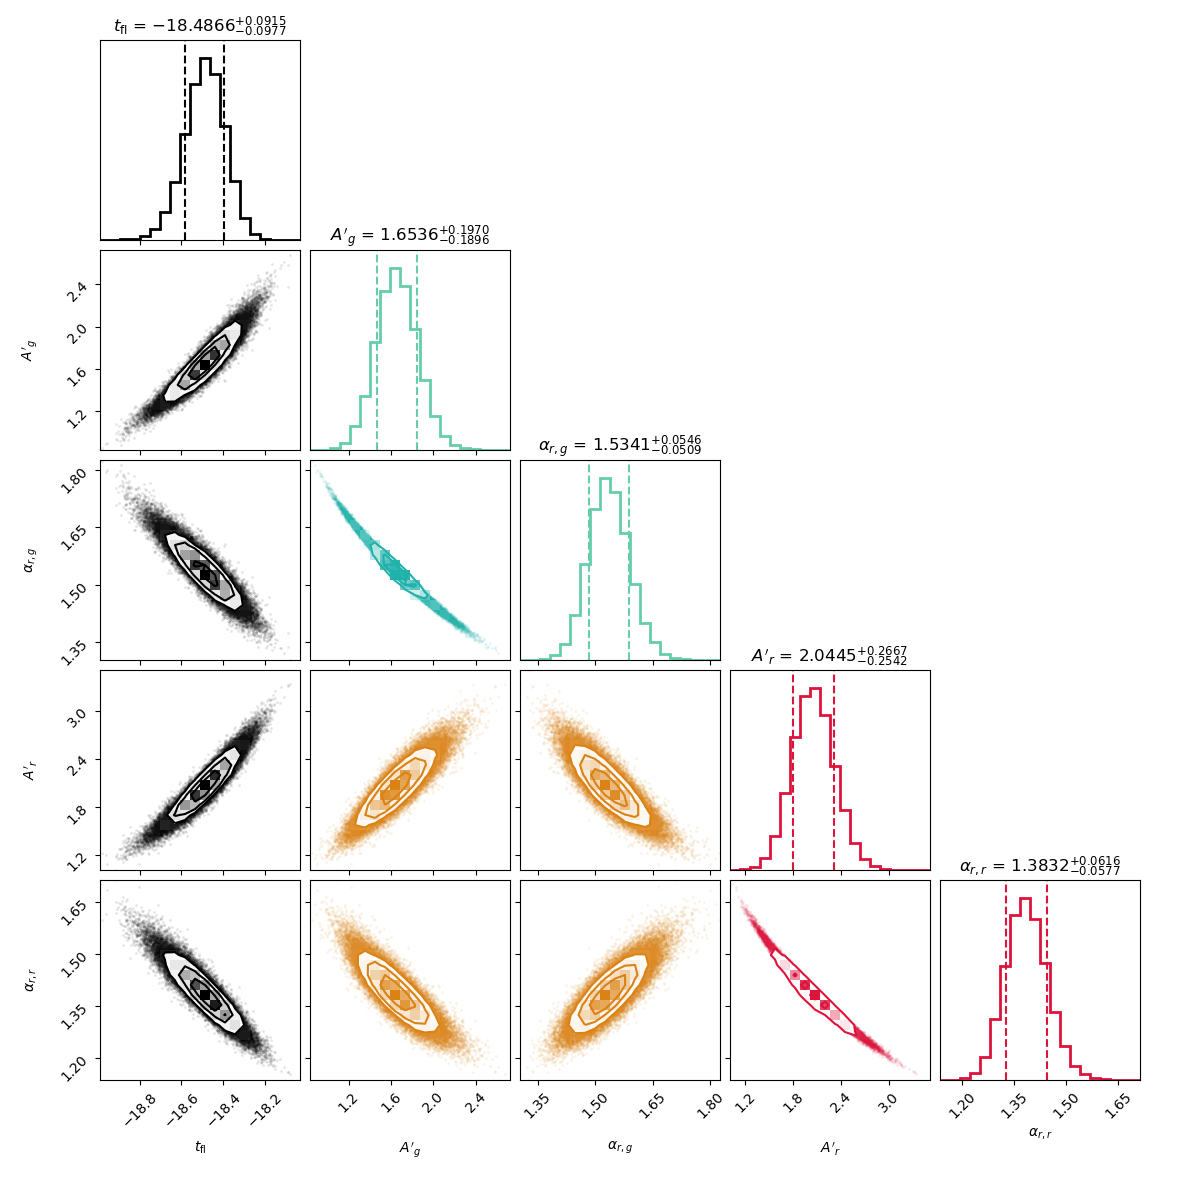
\includegraphics[width=1\linewidth]{./figures/ZTF18aasdted_corner.png}
    %
    \caption{Corner plot showing the posterior constraints on \tfl,
    $\alpha_g$, $\alpha_r$, and the respective constants of proportionality,
    $A_g$ and $A_r$ for ZTF18aasdted, a SN that is well-fit by the model. For
    clarity the $C_d$ and $\beta_d$ terms are excluded (in general they do
    not exhibit strong covariance with the parameters shown here as they are
    tightly constrained by the pre-SN observations). Marginalized
    one-dimentional distributions are shown along the diagonal, along with
    the median estimate and the 90\% credible region (shown with vertical
    dashed lines).}
    %
    \label{fig:good_corner}
\end{figure}

\begin{figure}
    \centering
    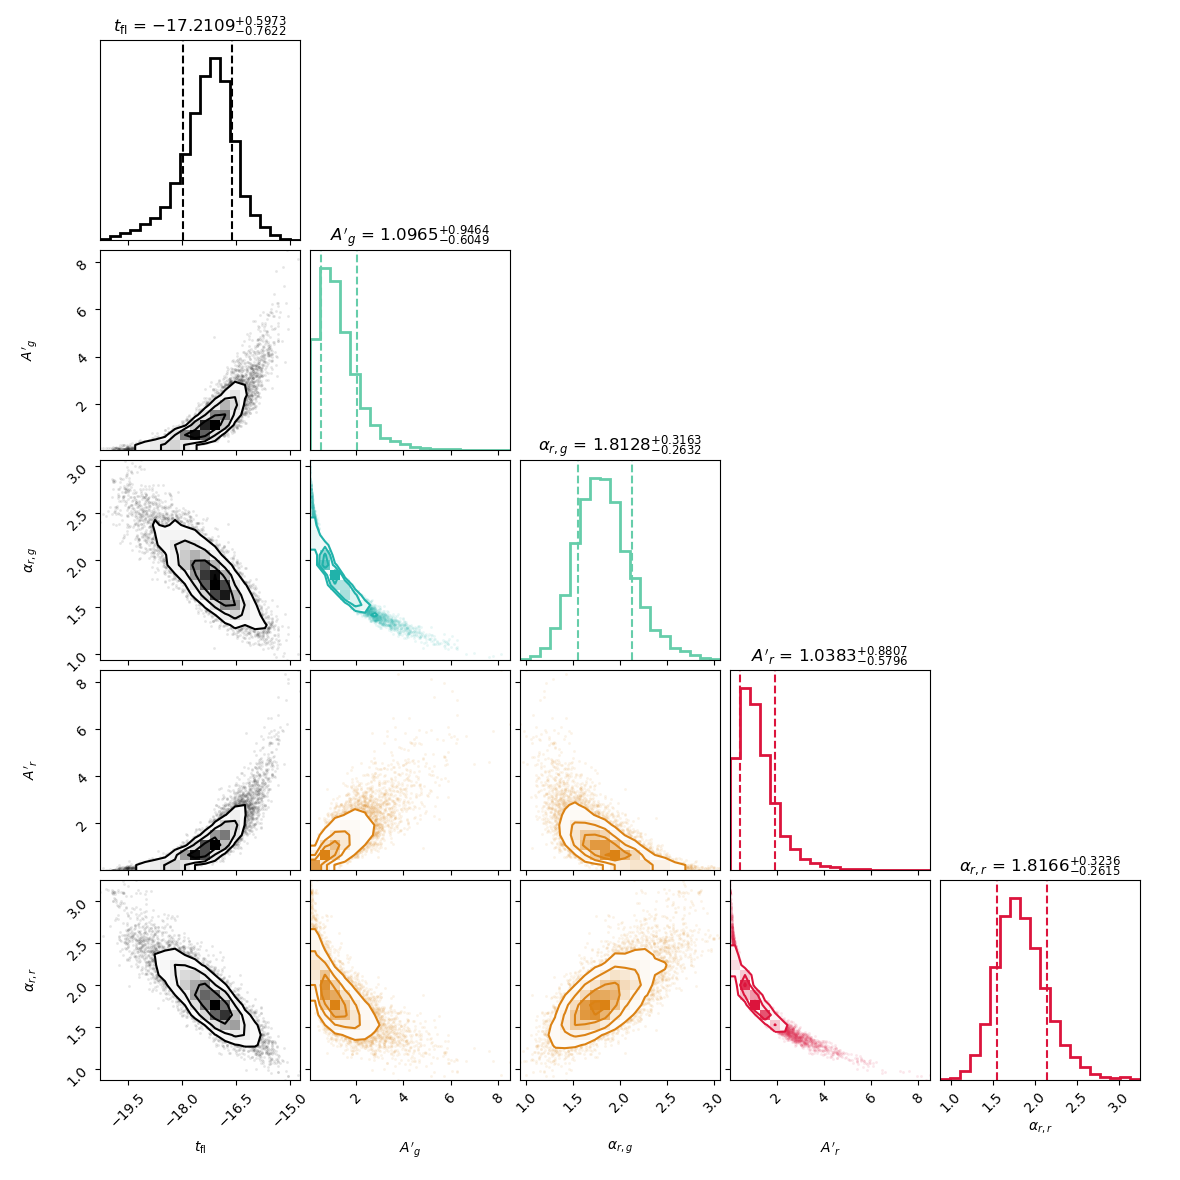
\includegraphics[width=1\linewidth]{./figures/ZTF18abukmty_corner.png}
    %
    \caption{Same as Figure~\ref{fig:good_corner} for ZTF18abukmty, a typical
    SN within our sample.}
    %
    \label{fig:median_corner}
\end{figure}

\begin{figure}
    \centering
    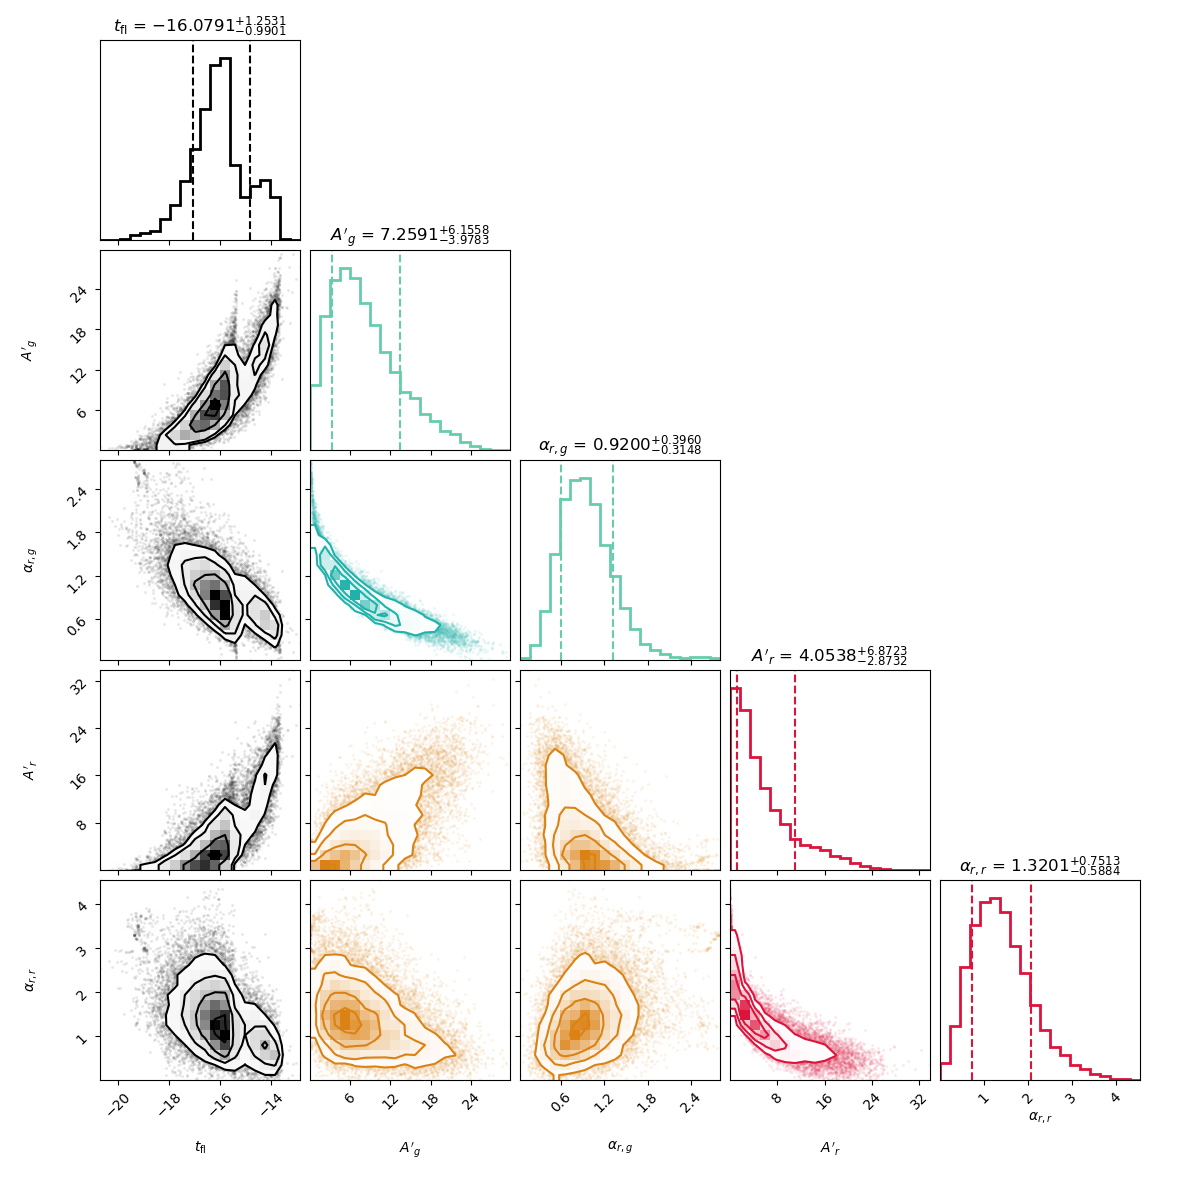
\includegraphics[width=1\linewidth]{./figures/ZTF18abkigee_corner.png}
    %
    \caption{Same as Figure~\ref{fig:good_corner} for ZTF18abkigee, a SN with
    poor constraints on the model parameters. The vast majority of SNe with
    poor model constraints feature gaps in the observational coverage, which
    in turn makes it difficult to contrain the model parameters. }
    %
    \label{fig:bad_corner}
\end{figure}



\section{Systematics\label{sec:systematics}}

\acknowledgements

Dan F-M? Will Farr?

\software{
         % \texttt{astropy} \citep{Astropy-Collaboration13},
          \texttt{scipy} \citep{Jones01}, 
          \texttt{matplotlib} \citep{Hunter07},
          \texttt{pandas} \citep{McKinney10},
          \texttt{emcee} \citep{Foreman-Mackey13},
          \texttt{corner} \citep{Foreman-Mackey16}
          }

%% For this sample we use BibTeX plus aasjournals.bst to generate the
%% the bibliography. The sample63.bib file was populated from ADS. To
%% get the citations to show in the compiled file do the following:
%%
%% pdflatex sample63.tex
%% bibtext sample63
%% pdflatex sample63.tex
%% pdflatex sample63.tex

\bibliography{/Users/adamamiller/Documents/tex_stuff/papers}
\bibliographystyle{aasjournal}

%% This command is needed to show the entire author+affiliation list when
%% the collaboration and author truncation commands are used.  It has to
%% go at the end of the manuscript.
%\allauthors

%% Include this line if you are using the \added, \replaced, \deleted
%% commands to see a summary list of all changes at the end of the article.
%\listofchanges

\end{document}

% End of file `sample63.tex'.
